\chapter{فصل مقدمه} 
\pagenumbering{arabic}
\newpage
\section{مقدمه:}

در دو دهه گذشته پیشرفت های عظیمی صورت گرفته است که به طور موثری اسپینترونیک و مغناطیسی را به یک نیروی قدرتمند که حوزه دستگاه های حافظه را شکل می دهد، ترکیب کرده است. مواد و پدیده‌های جدید با سرعت چشمگیری کشف می‌شوند و مجموعه‌ای رو به افزایش از بلوک‌های ساختمانی را فراهم می‌کنند که می‌توانند در طراحی دستگاه‌های کاربردی ترانزیستور مانند آینده مورد استفاده قرار گیرند.

تحولات دو دهه اخیر زمینه های متمایز اسپینترونیک و مغناطیس را در یک نیروی قدرتمند ترکیب کرده است. با شروع اثر مقاومت مغناطیسی غول پیکر \lr{(GMR)}، این میدان با اکتشافات جدید مانند اثر مقاومت مغناطیسی تونل بزرگ \lr{(TMR)}، سوئیچینگ اسپین انتقال گشتاور \lr{(STT)} و اخیراً، پدیده های مدار اسپینی بالا از جمله اثر سالن چرخش غول پیکر \lr{(GSHE)} و عایق های توپولوژیکی \lr{(TI)}.
دستگاه های حافظه اسپینترونیک مبتنی بر \lr{TMR} و \lr{STT} قبلاً تجاری شده اند در حالی که دستگاه های منطقی اسپینترونیک هنوز به طور فعال در حال بررسی هستند. مواد و پدیده های جدید با سرعت چشمگیری کشف می شوند که می توانند به عنوان مجموعه ای از "بلوک های ساختمانی" به طور مداوم در حال گسترش برای دستگاه های کاربردی پیچیده در نظر گرفته شوند.

\section{تئوری انتقال الکترونی و اسپینی در مواد دو بعدی:}
در این فصل، مفاهیم مورد نیاز برای درک ترابرد الکترونیکی و اسپین در مواد دو بعدی معرفی شده است. مقدمه ای بر خواص ترابرد الکترونیکی مواد دو بعدی بالک و جدا شده با مقدمه ای کوتاه بر اصل کار یک ترانزیستور اثر میدانی دنبال می شود. بعداً، مفهوم تزریق اسپین در مواد غیر مغناطیسی مانند گرافن نیز همراه با توضیح مختصری در مورد مدل دو کاناله برای انتقال اسپین در یک شیر اسپینی معمولی توضیح داده شده است. همچنین، مسائل مربوط به عدم تطابق هدایت و \lr{spin relaxation} ناشی از اتصالها مورد بررسی قرار می گیرد. متعاقباً، انتقال اسپین در گرافن، از جمله مفاهیم معادله انتشار اسپین، اندازه‌گیری دریچه اسپین ناجایگزیده و اندازه‌گیری تقدم اسپین \lr{Hanle} شرح داده می‌شود. بعداً، مکانیسم‌های مختلف \lr{spin relaxation} برای انتقال اسپین در گرافن معرفی شدند. در نهایت، مروری بر مطالعات نظری و تجربی در مورد انتقال اسپین در گرافن تک و دو لایه، در مجاورت با \lr{TMD}، ارائه شده است.

\subsection{ترابرد الکترونیکی در مواد 2 بعدی:}
در چهار دهه گذشته، مطالعات دقیقی برای درک انتقال بار الکترونیکی در نیمه هادی های لایه ای حجیم 1-3 انجام شده است. ساختار نوار الکترونیکی یک نیمه هادی لایه ای حجیم بسته به برهمکنش بین لایه ای بین لایه های دو بعدی آن تغییر می کند و این امر به طور قابل توجهی بر ترابرد الکترونیکی تأثیر می گذارد. علاوه بر این، در چنین نیمه‌رسانای لایه‌ای حجیم، می‌توان ویژگی‌های مختلف انتقال بار (ناهمسانگردی) را برای جهت‌های درون صفحه \lr{(x-y)} و خارج از صفحه \lr{(z)} انتظار داشت. در اینجا، جهت x-y مربوط به انتقال بار در طول و عرض مواد 2 بعدی حجیم است، در حالی که جهت z در امتداد ضخامت آن است. همچنین، با راه‌اندازی الکترواستاتیکی چنین مواد 2 بعدی حجیم از طریق کوپلینگ خازنی، می‌توان انتظار انباشتگی بالاتر حامل‌های بار در سطحی که نزدیک‌تر به دروازه است، در مقایسه با تخلیه حجیم به دلیل غربالگری بار بود.
اخیراً، مواد دو بعدی جدا شده از گرافن از گرافیت توده ای توسط \lr{Novoselov} و همکاران 7 به دست آمده است. با این حال، گرافن فاقد گاف نواری در ساختار نوار الکترونیکی خود است که برای تحقق \lr{FET} های مبتنی بر منطق ضروری است. این منجر به جستجوی دسته جدیدی از مواد دو بعدی شده است که نیمه رسانا هستند، مانند فسفر سیاه 5، \ce{MoS}28، \lr{germanane}9 و موارد دیگر. با انبوهی از مواد دوبعدی موجود که ویژگی‌های الکتریکی مختلف را ارائه می‌کنند، مطالعه انتقال بار الکترونیکی در نیمه‌رساناهای دو بعدی جدا شده افزایش یافته است. این علاقه زیاد به نیمه هادی های دو بعدی جدا شده عمدتاً به دلیل کاهش غربالگری حامل های بار در مقایسه با نیمه هادی های حجیم و به دلیل محصور شدن کوانتومی بیشتر حامل های بار به دلیل دو بعدی بودن آنها است.
\begin{figure*}[!ht]
    \centering
    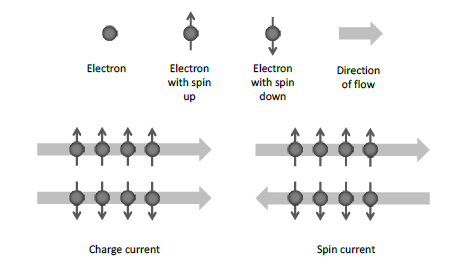
\includegraphics{spinchargecurent.png}
    \caption{برای یک جریان بار، الکترون های "بالا" و "پایین" در یک جهت جریان می یابند در حالی که برای یک جریان اسپین، الکترون های "بالا" و "پایین" در جهت مخالف جریان می یابند.}
    \label{fig:spinchargecurent}
\end{figure*}

\subsection{جریان شارژ و اسپین:}
الکترون یک ذره بنیادی یک اتم است که به دور هسته تشکیل شده از پروتون و نوترون می چرخد. بار الکتریکی یک الکترون منفی است و از مرتبه $1.60\times 10^19$ کولن است. الکترون همچنین دارای یک تکانه زاویه ای ذاتی است که اسپین نامیده می شود که مقدار آن $\pm\frac{1}{2}$ است بسته به این که: اگر اسپین الکترون در جهت عقربه های ساعت/بالا باشد (+) یا خلاف جهت عقربه های ساعت/پایین (-). زمانی گفته می‌شود که جریان بار در سیستمی جریان دارد که الکترون‌ها، هر دو با اسپین بالا و پایین، در یک جهت جریان داشته باشند که در شکل\ref{fig:spinchargecurent} نشان داده شده است. چگالی کل جریان شارژ ($j$) فقط سهم کل چگالی جریان اسپین بالا ($j\uparrow$) و پایین ($j\downarrow$) 
است، یعنی
\begin{equation}
    \vec{J}={\vec{J}}_{\uparrow }+{\vec{J}}_{\downarrow}
\end{equation}
در حالی که جریان اسپین از جریان اسپین بالا و پایین الکترون‌ها در جهت مخالف، همانطور که در شکل\ref{fig:spinchargecurent} نشان داده شده است، حاصل می شود. چگالی کل جریان اسپین ($j_s$) فقط تفاوت بین چگالی جریان اسپین بالا ($j\uparrow$) و پایین ($j\downarrow$) است، یعنی
\begin{equation}
    \vec{J}_{s} = \vec{J}_{\uparrow} - \vec{J}_{\downarrow}
\end{equation}
در حالی که پلاریزاسیون جریان اسپینی ($P_j$)،
\begin{equation}
    P_j = \frac{\vec{J}_{\uparrow} - \vec{J}_{\downarrow}}{\vec{J}_{\uparrow} + \vec{J}_{\downarrow}}
\end{equation}
\begin{figure*}[!ht]
    \centering
    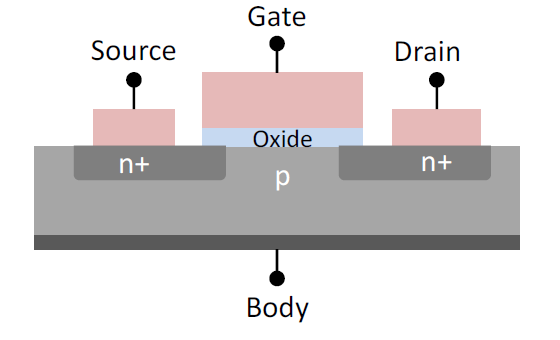
\includegraphics{MOSFET.png}
    \caption{نمای مقطعی یک ماسفت که دروازه، بدنه، منبع و پایانه تخلیه را نشان می دهد. گیت به صورت خازنی توسط یک لایه اکسید دی الکتریک نازک به کانال نیمه هادی کوپل شده است.}
    \label{fig:mosfet}
\end{figure*}
\section{ترانزیستور اثر میدانی نیمه هادی اکسید فلز:}
ترانزیستور اثر میدانی نیمه هادی اکسید فلز \lr{(MOSFET)} نوعی ترانزیستور اثر میدانی \lr{(FET)} است. همانطور که در شماتیک دستگاه شکل \ref{fig:mosfet} نشان داده شده است، این یک دستگاه سه ترمینالی است که از الکترودهای دروازه، منبع و تخلیه تشکیل شده است. یک ماسفت معمولی شامل یک نیمه هادی است که بین یک جفت الکترود فلزی به نام منبع و تخلیه متصل است. رسانایی نیمه هادی به طور خازنی توسط یک دروازه فلزی مدوله می شود که از طریق یک لایه اکسید نازک به کانال نیمه هادی متصل می شود، همانطور که در شکل \ref{fig:mosfet} نشان داده شده است. معمولا به صورت الکتریکی به زمین متصل می شود. ماسفت‌ها بسته به نوع حامل های بار در کانال نیمه هادی طبقه بندی می شوند، یعنی به عنوان نوع \lr{n} یا \lr{p} مربوط به انتقال بار الکترون یا حفره در کانال.
ترانزیستور نشان داده شده در شکل \ref{fig:mosfet} یک ماسفت سیلیکونی نوع \lr{n} است که در آن نیمه هادی سیلیکونی دوپ شده با حفره است. سیلیکون با دوپ بسیار الکترونی \lr{(n+)} به عنوان منبع و الکترودهای تخلیه استفاده می شود. دروازه معمولاً از پلی سیلیکون تشکیل شده است که مانع اکسید آن سیلیکون دی اکسید است. کاربرد اصلی ماسفت استفاده از آن به عنوان یک سوئیچ منطقی است که با روشن-خاموش کردن (که در منطق دیجیتال به صورت 1/0 نمایش داده می شود) جریان جاری در کانال نیمه هادی محقق می شود. برخی از عواملی که یک ماسفت خوب را مشخص می کند، ولتاژ عملیاتی آن، سرعتی که می توان جریان را روشن و خاموش کرد و ابعاد ترانزیستور است. ماسفت‌ها به طور مداوم برای دستیابی به عملکرد بهتر با مهندسی مواد و ابعاد کانال نیمه هادی، منبع، تخلیه و گیت در حال توسعه هستند.

\subsection{گرافن FET:}

گرافن اولین ماده دوبعدی کشف شده است [1]. کشف خصوصیات حیرت انگیز گرافن مجموعه ای از مواد جدید را به وجود آورده است که به عنوان "مواد دو بعدی" شناخته می شوند [2-4]. فرم های دو بعدی برای بسیاری از کاربردها یک منطقه نسبتاً هیجان انگیز و جدید است [5 ، 6]. معمولاً مواد دو بعدی دارای بسیاری از خصوصیات فیزیکی برجسته هستند که برای دستگاه های الکترونیکی ، مهندسی نانو ، تبدیل انرژی و فوتونیک امیدوار کننده است [7-11]. با توسعه سریع گرافن ، اخیراً مواد دو بعدی ، مانند فسفرن ، 
\lr{BN} ، ژرمن ، آنتیمونن ، سیلیسن ، آرسنن و دی الكوژنیدهای فلزات انتقالی ، مورد توجه گسترده قرار گرفته اند.

توده ای از مواد با ضخامت اتم از نظر تئوری پیش بینی یا سنتز شده است [12–16]. با کمال تعجب ، آنها ساختارهای متفاوتی از گرافن دارند ، این اختلاف از درجه های متفاوت خمیدگی حاصل می‌شود [17]. علاوه بر مواد دو بعدی لایه برداری شده از نمونه های بالک، برخی از مواد دوبعدی نیز می توانند از مواد بالک بدون فرم لایه ای تولید شوند ، مانند ترکیب بور تخت دوبعدی  \lr{GaN 2D} و هافنن [18 ، 19].

\begin{figure*}[!ht]
    \centering
    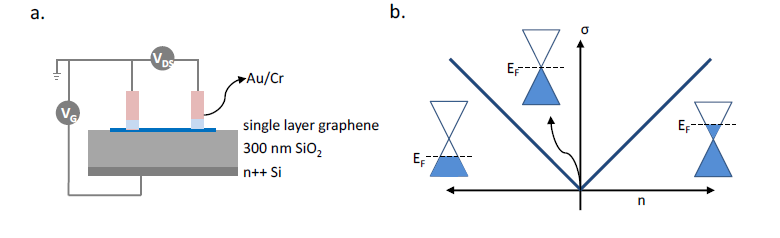
\includegraphics[width=\linewidth]{GrapheneFET.png}
    \caption{(الف). شماتیک دستگاه یک \lr{FET} با کانال گرافن بین الکترودهای منبع تخلیه و یک دروازه پشتی. (ب). طرحی از هدایت حامل بار ($\sigma$) گرافن \lr{FET} که تابعی از چگالی حامل بار \lr{(n)} ترسیم شده است. نمودار درونی – نواری گرافن با انرژی فرمی، $E_F$.}
    \label{fig:graphenefet}
\end{figure*}
تلاش دائمی در گسترش اثر میدان الکتریکی به فلزات صورت گرفته است. با این حال، این نیاز به فیلم‌های فلزی نازک اتمی دارد، زیرا میدان الکتریکی در فواصل کوتاه ($\le 1\;nm$) برای فلزات حجیم غربال می‌شود. علاوه بر این، غلظت حامل بار در یک فلز حجیم در مقایسه با بارهای سطحی که می تواند توسط میدان الکتریکی القا شود، زیاد است. اولین تلاش برای تحقق بخشیدن به اثر میدانی در یک لایه اتمی از گرافن نیمه فلزی توسط \lr{Novoselov} و همکاران انجام شد که در آن، \lr{FET} گرافن ساخته و مشخص شد و شماتیک دستگاه آن در شکل \ref{fig:graphenefet} نشان داده شده است. اعمال ولتاژ گیت \lr{($V_G$)} چگالی حامل بار \lr{(n)} و نوع حامل بار در گرافن را تغییر می دهد، همراه با تغییر موقعیت انرژی فرمی. می‌توان چگالی حامل بار القایی را با اندازه‌گیری جریان \lr{(IDS)} بین الکترودهای منبع تخلیه با جارو کردن ولتاژ \lr{(VDS)} اعمال شده در سراسر الکترودهای تخلیه منبع اندازه‌گیری کرد. هدایت اندازه گیری شده ($\sigma$)،$\sigma = ISD/VSD$، به عنوان تغییر در چگالی حامل بار همانطور که در شکل \ref{fig:graphenefet}(ب) نشان داده شده است، رسم شده است. محور مثبت n مربوط به چگالی حامل الکترون ($E_F$ در نوار رسانایی) و محور منفی n مربوط به چگالی حامل سوراخ ($E_F$ در باند ظرفیت) است. در حالی که در صفر است، از نظر تئوری انتظار می رود که چگالی حامل بار ($E_F$ در نقطه دیراک) در گرافن نداشته باشد. تغییر رسانایی از فرمول \lr{Drude} پیروی می کند 7، $\sigma = ne\mu$ (که \lr{e} بار الکترون است و $\mu$ تحرک حامل بار است). در نتیجه، تغییر خطی در $\sigma$ به عنوان تابعی از تغییر در n وجود دارد، همانطور که در شکل\ref{fig:graphenefet}(ب) نشان داده شده است. \lr{Novoselov} و همکاران 7 مقادیر معمول $\mu \approx 10000 cm^2/V·s$ و $n \approx 5 \times 10^{12} cm^{-2}$ را برای \lr{FET} های گرافنی خود اندازه گرفتند.
\begin{figure*}[!ht]
    \centering
    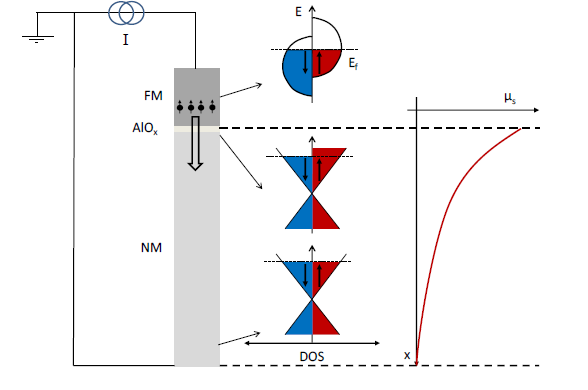
\includegraphics[width=\linewidth]{spininjection.png}
    \caption{تزریق اسپین از یک فرومغناطیس \lr{(FM)} به یک غیر آهنربا \lr{(NM)} همانطور که در قسمت سمت چپ شکل نشان داده شده است. پتانسیل شیمیایی اسپین در \lr{FM}، رابط )بین \lr{FM-\ce{AlOx}} و (\lr{NM}، و بخش عمده \lr{NM} در مرکز نشان داده شده است. فروپاشی نمایی انباشت اسپین القایی از رابط به بخش عمده \lr{NM} در قسمت سمت راست شکل نشان داده شده است.}
    \label{fig:spininjection}
\end{figure*}
\subsection{تزریق اسپین به مواد غیر مغناطیسی}:
در این بخش، فرآیند تزریق اسپینی از فرومغناطیس به غیر آهنربا به اختصار توضیح داده شده است. بعداً، مدل دو کاناله برای انتقال اسپین در یک شیر اسپینی معمولی توضیح داده شده است. در نهایت، موضوع عدم تطابق رسانایی و \lr{spin relaxation} ناشی از اتصالها مورد بررسی قرار می‌گیرد.
می توان با استفاده از فرومغناطیس \lr{(FM)} که دارای قطبش اسپین خالص است، به یک غیر آهنربا \lr{(NM)} مانند گرافن تزریق اسپین انجام داد. همانطور که در شکل \ref{fig:spininjection}نشان داده شده است، در یک فرومغناطیس، عدم تعادل در چگالی حالات برای الکترون های اسپین بالا و پایین در انرژی فرمی وجود دارد. این عدم تعادل منجر به تفاوت در رسانایی برای کانال های اسپین بالا و پایین می شود. برای یک سیستم انتشار، هدایت برای هر کانال اسپین، $\sigma\uparrow(\downarrow)$ را می توان به صورت زیر محاسبه کرد:
\begin{equation}
    \sigma_{\uparrow(\downarrow)} = g _{\uparrow(\downarrow)}(E_f) e^2 D_{\uparrow(\downarrow)}
    \label{eq:spintransport}
\end{equation}
که در آن، $g_{\uparrow(\downarrow)}$ چگالی حالات در انرژی فرمی $E_f$ و $D\uparrow(\downarrow)$ میزان انتشار هر کانال اسپین است. $D_{\uparrow(\downarrow)}$ به این صورت تعریف می شود،
\begin{equation}
    D_{\uparrow(\downarrow)}=\frac{v_{f\uparrow(\downarrow)}}{l_{mfp\uparrow(\downarrow)}}
\end{equation}
، که در آن $v_{F\uparrow(\downarrow)}$ سرعت فرمی، $l_{mfp\uparrow(\downarrow)}$ میانگین طول مسیر آزاد و ضریب 3 ابعاد یک سیستم سه بعدی را محاسبه می کند.
هنگامی که جریان از \lr{FM} به \lr{NM} جریان می یابد، عدم تعادل اسپین خالص \lr{FM} به \lr{NM} در فصل مشترک القا می شود که منجر به یک حالت غیر تعادلی در \lr{NM} می شود. عدم تعادل اسپین ناشی از تجمع اسپین ($\mu_s$) نامیده می شود. $\mu_s$ به عنوان اختلاف پتانسیل شیمیایی اسپین برای کانال‌های اسپین‌آپ ($\mu_{\uparrow}$) و کانال‌های اسپین پایین ($\mu\downarrow$) اندازه‌گیری می‌شود.$\mu_s=\frac{\mu{\uparrow}-\mu_{\downarrow}}{2}$.
علاوه بر این، هیچ عدم تعادل اسپینی در بخش عمده \lr{NM} وجود ندارد، که منجر به انتشار اسپین‌ها از رابط به قسمت عمده \lr{NM} می شود. همانطور که اسپین‌ها پخش می شوند، به دلیل برهم کنش آنها با ناخالصی‌ها یا فونون‌ها در بخش عمده \lr{NM}، تحت پراکندگی قرار می گیرند. از این رو، آنها   تحت \lr{realxation} قرار می گیرند. طول انتشار اسپین، $\lambda_s$ فاصله مشخصه ای است که در آن $\mu_s$ میرا می شود. $\lambda_s$ و $\mu_s$ به صورت، $\mu_s = \alpha\exp^{-x\lambda_s}$ مرتبط هستند. $\lambda_s$ مربوط به \lr{relaxation time} اسپین $\tau_s$ به عنوان $\lambda_s=\sqrt{D_s\tau_s}$ است، که در آن $D_s$ ضریب انتشار اسپین است. در مورد گرافن، جایی که برهمکنش الکترون-الکترون مکانیسم پراکندگی غالب است، $D_s=Dc$، جایی که $Dc$ ضریب انتشار بار است. می توان قطبش اسپین جریان ($P_{j}^{NM}$) \lr{NM} را به صورت $P_{j}^{NM} = \mu_sj_{NMRNM}$ نوشت، که در آن $j_{NM}$ چگالی جریان بار در \lr{NM} و $R_{NM}$ مقاومت موثر \lr{NM} است.
می توان هندسه دستگاه را در شکل \ref{fig:twochannelmodel} با قرار دادن یک لایه نازک \lr{FM} ساخت. مانند \ce{Co}، با ضخامت حدود 60 نانومتر و با نسبت طول به عرض 10. بالای گرافن یک لایه نازک اکسید از \ce{Al2O3} به عنوان یک مانع تونلی بین \lr{FM} و گرافن از برگشت اسپین های تزریق شده از گرافن به \lr{FM} جلوگیری می کند.
\begin{figure*}[!ht]
    \centering
    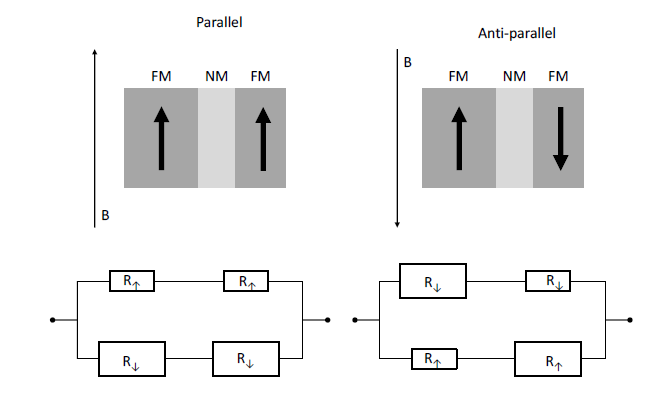
\includegraphics[width=\linewidth]{twochannelmodel.png}
    \caption{یک شیر اسپینی دو ترمینالی در شکل بالا با یک جفت FM که یک NM را ساندویچ می کند نشان داده شده است. شکل پایین مدل دو کاناله مربوطه را برای کانال اسپین بالا و پایین برای یک شیر اسپین دو ترمینالی نشان می دهد.}
    \label{fig:twochannelmodel}
\end{figure*}
\subsection{مدل دو کاناله:}
همانطور که در شکل\ref{fig:twochannelmodel}نشان داده شده است، یک غیر آهنربا \lr{(NM)} بین یک جفت فرومغناطیس \lr{(FM)} قرار می گیرد تا یک شیر اسپینی دو ترمینالی را تشکیل دهد. رسانایی برای الکترون های اسپین بالا و اسپین پایین در یک FM همانطور که در رابطه \ref{eq:spintransport} نشان داده شده است متفاوت است و بنابراین رسانایی کل FM $\sigma=\sigma_{\uparrow}+\sigma_{\downarrow}$ است، که $\sigma_{\downarrow}$ و $\sigma_{\uparrow}$ رسانایی برای اسپین کانال بالا و پایین به ترتیب هستند.

همانطور که در مدل مقاومت در شکل \ref{fig:twochannelmodel} نشان داده شده است، مقاومت برای کانال های اسپین بالا و پایین شیر اسپینی دو ترمینالی به عنوان یک مدل دو کاناله نشان داده شده است. یک میدان مغناطیسی خارجی برای مغناطیس کردن \lr{FM} در پیکربندی موازی اعمال می‌شود (فلش‌های شکل نشان‌دهنده جهت خالص مغناطیسی \lr{FM} هستند). در این هندسه، هنگامی که جریان از \lr{FM} چپ به \lr{FM} راست از طریق \lr{NM} می‌گذرد (مقاومت \lr{NM} نادیده گرفته می‌شود زیرا مستقل از اسپین است)، کانال اسپین‌بالا مقاومت پایینی را تجربه می‌کند در حالی که کانال اسپین پایین مقاومت بالایی را تجربه می‌کند. با این حال، سوئیچینگ مغناطیسی یکی از الکترودهای \lr{FM} از حالت بالا به پایین منجر به یک حالت ضد موازی می شود. در نتیجه، کانال‌های اسپین‌بالا و اسپین‌پایین یک مقاومت بالا و پایین را به صورت سری تجربه می‌کنند که در مدل مقاومت شکل \ref{fig:twochannelmodel}نشان داده شده است. بنابراین، مقاومت موثر برای الکترون‌های اسپین بالا در پیکربندی موازی کمتر از مقاومت در حالت ضد موازی است. در اصل، یک جریان قطبی اسپین از طریق شیر اسپینی در پیکربندی موازی وجود دارد، در حالی که یک انباشته خالص اسپین برای پیکربندی ضد موازی ایجاد می‌شود که به صورت افت ولتاژ در سراسر شیر اسپینی ظاهر می‌شود.

\subsection{عدم تطابق رسانایی و \lr{spin relaxation} ناشی از اتصال:}
تا اینجا، تزریق اسپین از یک \lr{FM} به یک \lr{NM} مورد بحث قرار گرفته است. با این حال، این تزریق اسپین می تواند به طور قابل توجهی تحت تاثیر عدم تطابق در هدایت اسپین برای یک \lr{FM} در یک \lr{NM} باشد. قبل از پرداختن به مشکل عدم تطابق رسانایی، باید مفهوم مقاومت اسپینی را ($R_s$) را درک کرد.
\begin{equation}
    R_{s}=\frac{\rho\lambda_{s}}{A}
\end{equation}
مقاومت اسپینی $R_s$، مقاومتی است که یک ماده برای جریان اسپین در آن ایجاد می کند. $\rho$ مقاومت، $\lambda_s$ طول انتشار اسپین و $A$ سطح مقطع ماده است. در مورد تزریق اسپین از یک \lr{FM} به یک \lr{NM}، مقاومت اسپین برای FM (RFM) کمتر از \lr{NM} ($R_{NM})$ است. منجر به جریان برگشتی اسپین‌ها به \lr{FM} می شود که در نهایت در FM به تعادل می رسد زیرا طول عمر اسپین‌ها در \lr{FM} کوتاه است. این جریان برگشتی اسپین‌ها از \lr{NM} به \lr{FM} به دلیل مشکل عدم تطابق رسانایی است.
می توان مشکل عدم تطابق رسانایی را با قرار دادن یک مانع رابط مقاومتی بالا بین \lr{FM} و \lr{NM} حل کرد. سد رابط از اکسیدهای فلزی مانند \ce{Al2O3}، \ce{TiO2} و \ce{MgO} تشکیل شده است. مقاومت مرتبط با مانع رابط \ce{Rb}، بالاتر از مقاومت \lr{NM} است. و علاوه بر این، \ce{Rb} به عنوان تابعی از ضخامت مانع قابل تنظیم است.
\section{بورفین:}
تحقیقات در مورد بور در ترکیبات مختلف را می توان به چند صد سال پیش بازگرداند ، زیرا بور دارای خاصیت فوق العاده ای است که می تواند تقریباً با تمام عناصر دیگر ترکیب شود.


در میان آنها ، نیترید بور شش ضلعی \lr{(h-BN)} یک ترکیب بند وسیع \lr{III-V} است. این یک ماده لایه ای با ساختار گرافیت مانند است که در آن شبکه های مسطح شش ضلعی \lr{h-BN} مرتباً روی هم انباشته می شوند. \lr{h-BN} دارای پایداری شیمیایی بالا ، خصوصیات فیزیکی عالی و هدایت حرارتی بالایی است [20–23].

در سال 2015 ، ورق بور \lr{2D} با موفقیت بر روی بسترهای نقره  \lr{(Ag)} ساخته شد [25]. مطالعه بوروفن محققان زیادی را در بسیاری از زمینه ها مانند علوم مواد ، فناوری نانو ، فیزیک ، شیمی و مواد تغلیظ شده جذب کرده است [13 ، 26 ، 27]. \lr{"Borophene"} نانو صفحه جدید بور با ضخامت اتم برای سنتز در مقیاس بزرگ است [28]. این سبک ترین ماده دوبعدی تا به امروز است. بوروفن همسایه گرافن است و بنابراین ، داشتن برخی از خصوصیات مشابه گرافن مطلوب است [29].

هر دو الکترون $\sigma$ و $\pi$ در بوروفن حالات الکترونیکی سطح فرمی را اشغال می کنند و آن را ابررسانا می کنند. فشار زیاد و فشار خارجی وجود ندارد. بوروفن می تواند بالاترین \lr{Tc} را در بین مواد \lr{2D} داشته باشد. برای ساختارهای بور\lr{2D} ، پیچیدگی شیمیایی و ساختاری ، خصوصیات الکترونیکی و پایداری به طور گسترده مورد بررسی قرار گرفته است [27 ، 30 ، 31].

اخیراً ، یک نانوساختار کاملاً فلزی مبتنی بر بور بر روی یک کریستال نقره با رسوب بخار فیزیکی ، به نام بوروفن، ساخته شده است [32–36]. فازهای زیادی از آلوتروپهای بور بالک و دوبعدی مانند $\alpha$ ، $\beta$ و غیره وجود دارد که از لحاظ نظری پیشنهاد شده اند [37–39]. 

اگرچه ، بور از مشارکت در تشکیل پیوندهای شیمیایی برای ایجاد یک شبکه لانه زنبوری پایدار جلوگیری می کند ، اما ممکن است یک ساختار مسطح پایدار توسط مخلوطی از لانه زنبوری همراه با واحدهای مثلثی ایجاد شود [42،43] این ساختار شامل دو اتم در سلول واحد اولیه است که \lr{2B:Pmmn} نامیده می شود، که در آن \lr{Pmmn} مخفف گروه فضایی 59 است که در یک سیستم بلوری \lr{orthorhombic} وجود دارد. \lr{Xu} و همکاران [44] یک ماده جدید دیراک را پیش بینی کرد: بوروفن هیدروژنه (بوروفان) ، مشخصه‌های دیراک را با سرعت قابل توجه فرمی نشان می دهد که تقریبا دو برابر گرافن است.

\section{ساختار رساله:}
 در این رساله با استفاده از محاسبات بر پایه‌ی تقریب تنگ‌بست و نظریه‌ی  رسانندگی لانداير و روش تابع گرین غیر تعادلی به بررسی‌های
 رفتارهای ساختار صفحات بورفین در رسانندگی برای طراحی ترانزیستورها یا دیگر ادوات اسپینتورنیک مثل دریچه اسپینی و... می‌پردازیم. در فصل دوم 
 این رساله به معرفی ساختار مذکور، ویژگیها و کاربردهای آن  پرداخته می‌شود. درفصل سوم، به
 بررسی روش تابع گرین غیر تعادلی و تقریب تنگ‌بست پرداخته می شود.
 فصل چهارم شامل نتایج کار است. سه قسمت اصلی است: در بخش اول، به علت آنکه در فرآیند تولد صفحات دو بعدی همواره انواع نقص‌ها وجود دارند،به بررسی ساختار بورفین $\beta_{12}$ حضور
 انواع نقصهای شبکه می‌پردازیم از جمله نقوص منفرد و نقص اندرسون.  در بخش دوم، خواص رسانش وابساوابسته  به اسپین را در نانونوار بورفین میدان ا، میدان تبادلی و برهمكنش بر‌پایه مدل تنگ بساات و تابع گرین بررساای میکنیم در بخش سوم، به بررسی رسانندگی در صفحات بورفین با هامیلتونی موثر و وجود پراکندگی کلاین تونلینگ را بررسی می‌کنیم. در پایان جمع بندی نتایج و پیشنهادهایی برای مطالعات آینده را در فصل پنج ارائه کردهایم.
 نتایج پژوهشهای انجام شده در این پایان نامه در مراجع [؟], [؟], [؟] به چاه رسیده است.